%**************************************************************************************
% License:
% CC BY-NC-SA 4.0 (http://creativecommons.org/licenses/by-nc-sa/4.0/)
%**************************************************************************************

\documentclass[notes]{beamer}

\mode<presentation> {

\usetheme{Madrid}

% Burnt orange
\definecolor{burntorange}{rgb}{0.8, 0.33, 0.0}
\colorlet{beamer@blendedblue}{burntorange}
% Pale yellow
\definecolor{paleyellow}{rgb}{1.0, 1.0, 0.953}
\setbeamercolor{background canvas}{bg=paleyellow}
% Secondary and tertiary palett
\setbeamercolor*{palette secondary}{use=structure,fg=white,bg=burntorange!80!black}
\setbeamercolor*{palette tertiary}{use=structure,fg=white,bg=burntorange!60!black}

% To remove the footer line in all slides uncomment this line
%\setbeamertemplate{footline}
% To replace the footer line in all slides with a simple slide count uncomment this line
%\setbeamertemplate{footline}[page number]

% To remove the navigation symbols from the bottom of all slides uncomment this line
%\setbeamertemplate{navigation symbols}{}
}

\usepackage{amsmath}
\usepackage{bm}
\usepackage{breqn}
\usepackage{cancel}
\usepackage{graphicx} % for figures
\usepackage{subcaption} % for subplots 
\usepackage[labelsep=space,tableposition=top]{caption}
\renewcommand{\figurename}{Fig.} 
\usepackage{cleveref}
\usepackage{caption,subcaption}% http://ctan.org/pkg/{caption,subcaption}
\usepackage{booktabs} % Allows the use of \toprule, \midrule and \bottomrule in tables
\usepackage{multirow}
\usepackage{tabularx}

% To print 2 slides on a page
%\usepackage{handoutWithNotes}
%\pgfpagesuselayout{2 on 1}[border shrink=2mm]
%----------------------------------------------------------------------------------------
%	TITLE PAGE
%----------------------------------------------------------------------------------------
% The short title appears at the bottom of every slide, the full title is only on the title page
\title[CE394M: Stresses - paths \& invariants]{CE394M: Stress paths and invariants} 
\author{Krishna Kumar} % name
\institute[UT Austin] % institution 
{
University of Texas at Austin \\
\medskip
\textit{
  \url{krishnak@utexas.edu}} % Your email address
}
\date{\today} % Date, can be changed to a custom date

\begin{document}

\begin{frame}
\titlepage % title page as the first slide
\end{frame}

\begin{frame}
 % Table of contents slide, comment this block out to remove it
 \frametitle{Overview}
  %Throughout your presentation, if you choose to use \section{} and \subsection{} 
  %commands, these %will automatically be printed on this slide as an overview 
 \tableofcontents
\end{frame}

%----------------------------------------------------------------------------------------
% slides
%----------------------------------------------------------------------------------------
\section{Stresses / strains in typical geotechnical lab tests}

%----------------------------------------------------------------------------------------
\begin{frame}
\frametitle{Stresses / strains}
\noindent
\fboxsep=0pt
\noindent
\begin{minipage}[t]{0.65\linewidth}
	\textbf{1D consolidation / simple shear}
	\mode<beamer>{
		\begin{itemize}
			\item Zero lateral strain ($\varepsilon_{22} = \varepsilon_{33} = 0$
			)
			\item Stresses: $\sigma$ and $\tau$
			\item Strains: $\varepsilon_{11} = \varepsilon_{v}$ and $\gamma$
		\end{itemize}
	}
	\mode<handout>{
		\vspace{2cm}
	}
	\textbf{2D plane strain}
	\mode<beamer>{
		\begin{itemize}
			\item Zero lateral strain ($\varepsilon_{22} = \gamma_{12} = \gamma_{23} = 0$
			)
			\item Stresses: $s$ and $t$
			\item Strains: $\varepsilon_{v}$ and $\varepsilon_{\gamma}$
		\end{itemize}
	}
	\mode<handout>{
		\vspace{2cm}
	}
	\textbf{3D general (axi-symmetric as a special case)}
	\mode<beamer>{
		\begin{itemize}
			\item Stresses: $p$ and $q$
			\item Strains: $\varepsilon_{v}$ and $\varepsilon_{s}$
		\end{itemize}
	}
	\mode<handout>{
		\vspace{1.5cm}
	}

\end{minipage}%
\hfill
\begin{minipage}[t]{0.35\linewidth}
	\begin{figure}
		\includegraphics[width=\textwidth]{figs/stresses.png}
	\end{figure}
\end{minipage}	
\end{frame}

%----------------------------------------------------------------------------------------
\begin{frame}
\frametitle{1D simple shear}
\mode<beamer>{
	\begin{enumerate}
		\item No lateral strain
		\item Constant normal effective stress $\sigma_v^\prime$
		\item Increasing shear strain $\gamma$
		\item Measure shear resistance $\tau$
		\item Measure volumetric strain $\varepsilon_v$ or void ratio $e = e_0 - (1 + e_0)\varepsilon_v$
		\item \textbf{No information for the lateral direction}
	\end{enumerate}
}
\mode<handout>{
	\vspace{3cm}
} 
\begin{figure}
	\includegraphics[width=\textwidth]{figs/simple-shear.png}
\end{figure}
\end{frame}

%----------------------------------------------------------------------------------------
\begin{frame}
\frametitle{2D plane strain / Mohr-Coulomb model}
\textbf{Stresses and strains: independent components}
\noindent
\fboxsep=0pt
\noindent
\begin{minipage}[t]{0.65\linewidth}
\mode<beamer>{
	\begin{enumerate}
		\item Mean stress: $s = (\sigma_{I} + \sigma_{III}) / 2$ and $s^\prime = s - u$
		\item Volumetric strain: $\varepsilon_v = (\varepsilon_I + \varepsilon_{III})$
		\item Deviatoric / shear stress: $t = (\sigma_I - \sigma_{III}) / 2$ and $t^\prime = t$.
		\item Deviatoric / shear strain: $\varepsilon_\gamma = (\varepsilon_I - \varepsilon_{III})$
		\item Work increment:
		\begin{equation*}
			\delta W = \sigma_I^\prime \delta \varepsilon_I + \sigma_{III}^\prime \delta \varepsilon_{III} = s^\prime \delta \varepsilon_v + t \delta \varepsilon_\gamma
		\end{equation*}
		\item $s$ and $t$ are often used to derive parameters for Mohr-Coulomb model because it only considers $\sigma_I$ and $\sigma_{III}$ and not $\sigma_{II}$.
	\end{enumerate}
}
\mode<handout>{
	\vspace{3cm}
} 

\end{minipage}%
\hfill
\begin{minipage}[t]{0.35\linewidth}
\begin{figure}
	\includegraphics[width=\textwidth]{figs/plane-strain-stresses.png}
\end{figure}
\end{minipage}
\end{frame}

\note{
 Principal stresses	$\sigma_I > \sigma_{II} > \sigma_{III}$. This equation holds good and is the definition of $\sigma$ in principal stress notations, i.e., $I > II > III$.
 
 No shear stresses on these planes.
}

%----------------------------------------------------------------------------------------
\begin{frame}
\frametitle{2D Mohr circle}
\mode<beamer>{
\begin{figure}
	\includegraphics[width=\textwidth]{figs/mohr-circle.png}
\end{figure}
}
\mode<handout>{
\vspace{6cm}
}
\end{frame}

%----------------------------------------------------------------------------------------
\begin{frame}
\frametitle{Mohr circle to 2D stress components}
Successive Mohr circles and stress path for constant $\sigma_3$ and increasing $\sigma_1$:
\mode<beamer>{
\begin{figure}
	\includegraphics[width=\textwidth]{figs/mohr-circle-ts.png}
\end{figure}
}
\mode<handout>{
\vspace{6cm}
}
\end{frame}

%----------------------------------------------------------------------------------------
\begin{frame}
\frametitle{Effect of $\sigma_{II}$}
Bishop (1966) defined \textbf{b-value}: \mode<beamer>{$b = (\sigma_{II} - \sigma_{III}) / (\sigma_I - \sigma_{III})$, where $\sigma_I > \sigma_{II} > \sigma_{III}$. Triaxial compression $b = 0$, triaxial extension $b = 1$. 

Typically $\phi^\prime_{ps} = (1.05 - 1.15)\phi^\prime_{tx}$.
}
\begin{figure}
	\includegraphics[width=0.58\textwidth]{figs/friction-ps-tx.png}
	\caption*{Effect of $\sigma_{II}$ on friction angle (Kulhawy and Mayne, 1990)}
\end{figure}
\end{frame}
\note{$\sigma_{II}$ do have an effect on soil behavior. For example, the friction angle depends on the loading condition: triaxial compression, plane-strain, triaxial extension and others $\dots$., The effect of $\sigma_{II}$ can be measured using
true triaxial apparatus or hollow cylinder torsional
shear apparatus. In general, the peak friction
angle increases 10 to 15 percent from b = 0 (triaxial
compression) to b = 0.3 to 0.4 (plane strain), and it
stays constant or slightly decreases as b reaches 1 (tri-axial extension).

The variation of measured friction angle with
changes in $\sigma_{II}$ can be attrib-
uted to the effects of different mean stress and stress
anisotropy on the dilatancy and particle rearrangement
contributions to the total strength. For given maximum
and minimum principal stresses, the TXE
conditions have the largest mean effective stress,
whereas the triaxial compression conditions have the
smallest mean effective stress. The higher confinement
for triaxial extension and plane strain conditions contributes to the increasing friction angle for these conditions. (Mitchell and Soga., 2005)
}

%----------------------------------------------------------------------------------------
\begin{frame}
\frametitle{Effect of $\sigma_{II}$ on friction}
\begin{figure}
	\includegraphics[width=0.65\textwidth]{figs/friction-bvalue.png}
	\caption*{Chapter 11., Mitchell and Soga, 2005}
\end{figure}
\end{frame}


%----------------------------------------------------------------------------------------
\begin{frame}
\frametitle{Effect of $\sigma_{II}$ on friction}
	Various models fit the experimental data showing the intermediate stress effect.
	Lade and Duncan (1975)
	\begin{equation*}
		\frac{I_1^3}{I_3} = const
	\end{equation*}
	
	Matsuoka and Nakai (1974)
	\begin{equation*}
		\frac{I_1 I_2}{I_3} = const
	\end{equation*}
	
	\begin{align*}
		I_1 &= \sigma_1 + \sigma_2 + \sigma_3 \\
		I_2 &= \sigma_1\sigma_2 + \sigma_2 \sigma_3 + \sigma_3 \sigma_1\\
		I_3 &= \sigma_1\sigma_2\sigma_3
	\end{align*}
Matsuoka and Nakai's model gives the same friction angle for compression and extension, whereas Lade and Duncan's model gives the ratio of the TXE friction angle ($\phi_{TXE}^\prime$) to the TXC friction angle ($\phi_{TXC}^\prime$) to be 1.08 at $\phi_{TXC}^\prime = 20^o$ to 1.15 at $\phi_{TXC}^\prime = 40^o$. 
\end{frame}
\note{Given the large scatter in the published experimental data, it is not possible to conclude that one model is better than the ohter. 
}


%----------------------------------------------------------------------------------------
\begin{frame}
\frametitle{Triaxial stresses and strains: independent components}
\noindent
\fboxsep=0pt
\noindent
\begin{minipage}[t]{0.65\linewidth}
	\mode<beamer>{
		\begin{itemize}
			\item We split the stress system into:
			\begin{itemize}
				\item purely volumetric deformation `\textit{p}'
				\item purely distortional deformation `\textit{q}'
			\end{itemize}
			\item Mean stress: 
			\begin{equation*}
			p = (\sigma_a + 2\sigma_r) / 3 \quad  p^\prime = p - u
			\end{equation*}
			\item Volumetric strain: $\varepsilon_v = (\varepsilon_a + 2 \varepsilon_r)$
			\item Deviatoric / shear stress (purely distortional deformation):
			\begin{equation*}
				q = (\sigma_a - \sigma_r) \quad q^\prime = q
			\end{equation*}
			\item Deviatoric / shear strain: $\varepsilon_s = 2/3 (\varepsilon_a - \varepsilon_r)$
		\end{itemize}
	}
	\mode<handout>{
		\vspace{3cm}
	}
\end{minipage}%
\hfill
\begin{minipage}[t]{0.35\linewidth}
	\begin{figure}
		\includegraphics[width=\textwidth]{figs/triaxial.png}
	\end{figure}
\end{minipage}	
\end{frame}


%----------------------------------------------------------------------------------------
\begin{frame}
\frametitle{Triaxial deviatoric strain}
	\begin{itemize}
		\item Deviatoric / shear strain: $\varepsilon_s = 2/3 (\varepsilon_a - \varepsilon_r)$
		\item Why 2/3?:
		\mode<beamer>{	
		\item Work equation: $\delta W = p^\prime \delta \varepsilon_v + q^\prime \delta \varepsilon_s$
		\begin{align*}
			\delta W & = \sigma_1^\prime \delta \varepsilon_1 + \sigma_2^\prime \Delta \varepsilon_2 + \sigma_3^\prime \Delta \varepsilon_3  = \sigma_a^\prime \delta \varepsilon_a + 2 \sigma_r^\prime \delta \varepsilon_r\\
			\delta W & = (1/3 \sigma_a^\prime + 2/3 \sigma_r^\prime)(\varepsilon_a + 2 \varepsilon_r) + (\sigma_a^\prime - \sigma_r^\prime)(2/3)(\varepsilon_a - \varepsilon_r) \\
			& = \sigma_a^\prime \delta \varepsilon_a + 2 \sigma_r^\prime \delta \varepsilon_r 
		\end{align*}
	}
	\mode<handout>{
	\vspace{3cm}
	}
	\end{itemize}

\end{frame}


%----------------------------------------------------------------------------------------
\begin{frame}
\frametitle{Triaxial stress - strain relationship}
Relationship in terms of axial and radial direction:
\begin{equation}
	\begin{bmatrix}
		\varepsilon_a \\
		\varepsilon_r \\
	\end{bmatrix}%
	=%
	\frac{1}{E}%
	\begin{bmatrix}
		1 & - 2\nu\\
		-\nu & (1-\nu)\\
	\end{bmatrix}%
	\begin{bmatrix}
		\sigma_a \\
		\sigma_r \\
	\end{bmatrix}
\end{equation}
\mode<beamer>{	
Relationship in terms of `\textit{p}' and `\textit{q}':
\begin{equation}
	\begin{bmatrix}
		p \\
		q \\
	\end{bmatrix}%
	=%
	\begin{bmatrix}
	1/3 &  2/3\\
	1   & -1\\
	\end{bmatrix}%
	\begin{bmatrix}
	\sigma_a \\
	\sigma_r \\
	\end{bmatrix}%
	\quad
	\text{ invert }
	\rightarrow
	\begin{bmatrix}
		\sigma_a \\
		\sigma_r \\
	\end{bmatrix}%	
	\begin{bmatrix}
		1   &  2/3\\
		1   & -1/3\\
	\end{bmatrix}%
	\begin{bmatrix}
		p \\
		q \\
	\end{bmatrix}%
\end{equation}

Strain:
\begin{equation}
	\begin{bmatrix}
		\varepsilon_p \\
		\varepsilon_q \\
	\end{bmatrix}%
	=%
	\begin{bmatrix}
		1   &  2\\
		2/3   & -2/3\\
	\end{bmatrix}%
	\begin{bmatrix}
		\varepsilon_a \\
		\varepsilon_r \\
	\end{bmatrix}%
\end{equation}
}
\mode<handout>{
	\vspace{5cm}
}
\end{frame}


%----------------------------------------------------------------------------------------
\begin{frame}
\frametitle{Mohr circle to 3D stress components}
Successive Mohr circles and stress path for constant $\sigma_3$ and increasing $\sigma_1$:
\mode<beamer>{	
\begin{figure}
	\includegraphics[width=\textwidth]{figs/mohr-circle-pq.png}
\end{figure}
}
\mode<handout>{
\vspace{6cm}
}
\end{frame}


%----------------------------------------------------------------------------------------
\begin{frame}
\frametitle{Stress paths p-q}
Different stress paths for initially hydrostatic stress conditions:
\mode<beamer>{	
	\begin{figure}
		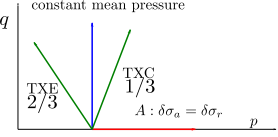
\includegraphics[width=\textwidth]{figs/stress-paths-pq.png}
	\end{figure}
}
\mode<handout>{
	\vspace{6cm}
}
\end{frame}

%----------------------------------------------------------------------------------------
\begin{frame}
\frametitle{Triaxial compression}
TXC with constant back pressure $u_o$ (TSP: Total stress path; ESP: Effective stress path)
\mode<beamer>{	
	\begin{figure}
		\includegraphics[width=0.8\textwidth]{figs/txc-tsp-esp.png}
	\end{figure}
}
\mode<handout>{
	\vspace{6cm}
}
\end{frame}

%----------------------------------------------------------------------------------------
\begin{frame}
\frametitle{Triaxial compression undrained: loose v dense}
\mode<beamer>{	
	\begin{figure}
		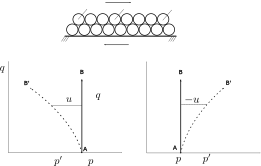
\includegraphics[width=0.85\textwidth]{figs/tx-undrained-pwp.png}
		\caption*{Total and effective stress paths for undrained triaxial test: (a) on soil that wishes to contract as it is sheared, and (b) on soil that wishes to expand as it is sheared.}
	\end{figure}
}
\mode<handout>{
	\vspace{6cm}
}
\end{frame}

%----------------------------------------------------------------------------------------
\begin{frame}
\frametitle{Triaxial compression drained: loose}
\begin{figure}
	\includegraphics[width=0.55\textwidth]{figs/tx-drained-loose.png}
	\caption*{Loose Sacramento River sand: (a) principal stress ratio versus
		axial strain; (b) volumetric strain versus axial strain (Lee, 1965).}
\end{figure}
\end{frame}

%----------------------------------------------------------------------------------------
\begin{frame}
\frametitle{Triaxial compression drained: dense}
\begin{figure}
	\includegraphics[width=0.43\textwidth]{figs/tx-drained-dense.png}
	\caption*{Dense Sacramento River sand: (a) principal stress ratio versus
		axial strain; (b) volumetric strain versus axial strain (Lee, 1965).}
\end{figure}
\end{frame}

%----------------------------------------------------------------------------------------
\begin{frame}
\frametitle{Triaxial compression drained: loose v dense}
\begin{figure}
	\includegraphics[width=0.35\textwidth]{figs/tx-drained-loose-dense.png}
	\caption*{Triaxial tests on “loose” and “dense” specimens of a typical sand: (a) stress-strain curves; (b) void
		ratio changes during shear (Hirschfeld, 1963).}
\end{figure}
\end{frame}

\end{document}
